\chapter{Label inference}
\section{Problem Statement}\label{\positionnumber}
A lot of data contains implicit regularities and structure~\cite{mitchell2006discipline}~\cite{carlsson2009topology} that are not reflected explicitly by the data model.\\
When focusing on data objects\note{or data instances, data points, elements of the sample, $\dots$} or nodes in terms of the property graph model there is often an implicit hierarchy of sub-types given a label. Such an implicit type hierarchy may provide further insights about the data as it may e.g. help in estimating cardinalities during query optimization, when keeping further statistics about the latent class distribution. \\

\margincode{code/business_ex.json}{businesex}{An example business object from the yelp data set}{text}{1cm}

For example in the yelp data set, the businesses may be further categorized in e.g. restaurants, spas, shopping malls, etc. One may further subdivide the restaurants by additional properties and features like cooking style (italian, asian, burgers, $\dots$) or  by location (italian restaurants in New York, asian restaurants in Manhatten). See lst. \ref{lst:businesex} for an example object. \\
The below example is motivated by the yelp data set. In the yelp data set instances are assigned categories by users of the yelp system. Inspecting them shows frequently category label distributions like in Tab. \ref{tab:running_ex}: \\
\begin{table}[htp]
     \centering
     \begin{tabular}{c c} \toprule
            Node.name & Node.labels \\ \midrule
            Fernando's & restaurant, italian \\ 
            Arche & restaurant, vietnamese \\ 
            ZumElefanten & restaurant, thai \\ 
            CampusCafe & cafe, wifi \\ 
            Endlicht & cafe, latenight \\ 
            Pano & cafe, breakfast \\
            Lago & shopping, mall \\ 
            Seerhein Center & shopping, cheap \\ 
            Seepark & Shopping, expensive \\ \bottomrule
        \end{tabular}
    \caption{A fictive example of business and user-defined associated labels.}
    \label{tab:running_ex}
\end{table}{}
Which may be visualized as hierarchy like in fig. \ref{fig:ex_hier}. \\
\fig{img/ex_hierarchy}{ex_hier}{The hierarchy that is implicit in the labels of the example in tab.\ref{tab:running_ex}}{1} \\
 In practice the categories are just informal strings, there is no notion of this structure in the current representation of the property graph model. In order to leverage this implicit hierarchy it needs to be made explicit. \\
 
Given a property graph model-based database, how can one extract such a hierarchy?
Finding classes or in other terms subsets of the input is what is addressed by clustering methods. \\
In order to infer a classes for nodes from a property graph model-based database, one may take various information into account: 
\begin{itemize}
    \item the user-defined labels only
    \item the properties of the node
    \item per node structural features of the underlying graph
    \item the properties of the relationships
    \item further constructed features based on previous steps
\end{itemize}
As briefly mentioned in chapter 2, different algorithms yield different clusterings as well as the same clustering algorithm with different features and parameters yields different clusterings. Thus in order to find a suitable hierarchy the following steps will be subsequently performed:
\begin{enumerate}
    \item Find a suitable clustering algorithm using a minimal feature set and different parameters to cover the space of algorithms and parameters as extensively as feasible.
    \item Find a suitable feature vector leveraging the graph structure
    \item Specify a pipeline to unify the above results
\end{enumerate}
Each step has it's own requirements and objectives that are addressed in the subsequent sections. \\
%% TODO reformulate as 2 step process

\section{Overview}\label{\positionnumber}
\fig{img/pipeline.png}{pipeline}{The pipeline used to evaluate the clustering approaches}{1}
The selection of a fitting algorithm has three main requirements:
\begin{itemize}
    \item Memory usage: data bases need a certain amount of memory to work and memory is always the main performance bottleneck for databases
    \item Adaptive to nominal and numeric data: Most databases support a couple of data types, that may be summarized as either nominal (string, characters, booleans, $\dots$) or numeric (integer, long, floats, $\dots$), i.e. the clustering algorithm needs to be able to support both kinds of data.
    \item Noise detection and tolerance: As there are frequently missing fields in data records the clustering algorithm should be tolerant to noise and detect noisy instances. E.g. in the yelp data set the maintenance of the business categories and other data is dependent on the support of the community around yelp and the owner of the business.
\end{itemize}
An overview of the Algorithm evaluation pipeline can be seen in fig. \ref{fig:pipeline}
In order to evaluate a wide range of algorithms, a pipeline is used that uses the interface for clustering algorithms specified in \fullref{clustering}. \\
The interface looks then like \ref{endtoend}
\begin{algorithm}[htp]
    \KwIn{Set of Objects $O$, set of sets of Attributes $A = \{A_{o_0}, A_{o_1}, \dots \}$}
    \Parameters{Parameters P to the implementation if necessary}
    \KwOut{A Taxonomy of $O$} 
\caption{Pipeline}\label{endtoend}
\end{algorithm}
% TODO generalize


\section{The Label-based Pipeline}
\subsection{Encoding labels as vectors}
\begin{algorithm}[htp]
    \KwIn{Set of Objects $O$, set of sets of Attributes $A = \{A_{o_0}, A_{o_1}, \dots \}$}
    \Parameters{No Parameters}
    \KwOut{A matrix $M$ of shape $|O| \times |A|$ with $m_{o,a} \in \{0, 1\}$} 
    \Begin{
        $M \rightarrow zeros(|O|, |A|)$\;
        \For{Object o in O} {
            \For{Attribute a in A}{
                \If{$a \in A_o$}{
                    $M[o,a] = 1$\;
                }
            }
        }
    }
\caption{Vectorize Labels}\label{vect}
\end{algorithm} 
Most clustering algorithms take a feature vector as input, that is a matrix of reals on some metric space. Character strings need to be transformed to comply with this requirement. Vectorization builds a matrix representation, given a set of string attributes per object.
One can easily do this by constructing the relation $I$, that given the set of objects $O$ and a set of attributes per object is defined as $1$ if object $o$ has attribute $a$ in it's set, $0$ otherwise.
Consider the example given in tab. \ref{tab:running_ex}. The vectorized representation of the example in tab. \ref{tab:running_ex} is given in tab. \ref{tab:vect_running_ex}
\begin{table}[htp]
 \begin{adjustwidth}{-4cm}{0cm}  
     \centering
     \begin{tabular}{|c|c|c|c|c|c|c|c|c|c|c|c|c|} \hline
            Node.name & rest & ital & viet & thai & cafe & wifi & late & brea & shop & mall & chea & expe \\ \hline \hline
            Fernando's      & 1 & 1 & 0 & 0 & 0 & 0 & 0 & 0 & 0 & 0 & 0 & 0  \\  \hline
            Arche           & 1 & 0 & 1 & 0 & 0 & 0 & 0 & 0 & 0 & 0 & 0 & 0  \\  \hline
            ZumElefanten    & 1 & 0 & 0 & 1 & 0 & 0 & 0 & 0 & 0 & 0 & 0 & 0  \\ \hline
            CampusCafe      & 0 & 0 & 0 & 0 & 1 & 1 & 0 & 0 & 0 & 0 & 0 & 0 \\ \hline
            Endlicht        & 0 & 0 & 0 & 0 & 1 & 0 & 1 & 0 & 0 & 0 & 0 & 0 \\ \hline
            Pano            & 0 & 0 & 0 & 0 & 1 & 0 & 0 & 1 & 0 & 0 & 0 & 0 \\ \hline
            Lago            & 0 & 0 & 0 & 0 & 0 & 0 & 0 & 0 & 1 & 1 & 0 & 0 \\ \hline
            Seerhein Center & 0 & 0 & 0 & 0 & 0 & 0 & 0 & 0 & 1 & 0 & 1 & 0 \\ \hline
            Seepark         & 0 & 0 & 0 & 0 & 0 & 0 & 0 & 0 & 1 & 0 & 0 & 1\\ \hline
        \end{tabular}
    \caption{A vector representation of the example from tab. \ref{tab:running_ex} corresponding to $I$}
    \label{tab:vect_running_ex}
    \end{adjustwidth}
\end{table}{} \\


\subsection{Compute Distance Matrix}
Given that we cluster sets of labels, a suitable distance is the Jacquard distance, that is a similarity measure for sets~\cite{DBLP:journals/corr/Kosub16}. If we consider the constraint that all sets are characterized by a vector of the same length we get that the Jacquard distance yields the same order as the Manhattan distance. \\
The proof is straightforward: 
\[ \textbf{Jarrad Distance} d_J (A,B) = \frac{(A \cup B) - (A \cap B)}{A \cup B} = \]
\begin{algorithm}[htp]
    \KwIn{linkage matrix $lM$}
    \Parameters{None}
    \KwOut{A taxonomy of $O$} 
    \Begin{
        previousRow $\leftarrow [-1, -1, -1]$\;
        taxonomy $\leftarrow$ new Map\;
        cluster $\leftarrow$ new Set\;
        distance $\leftarrow$ -1\;
        consecutive = False\;
        \For{row in $lM$}{
            \If{(row[0] == previousRow[0] or row[1] == previousRow[1])  and row[2] == previousRow[2]}{
                \If{taxonomy is not empty and not consecutive}{
                    taxonomy.removeLast()\;
                    cluster.add(previousRow[0], previousRow[1])\;
                }
                 distance $\leftarrow$ row[2]\;
                 cluster.add(row[0], row[1])\;
                 consecutive $\leftarrow$ True\;
            }{
                \If{consecutive}{
                    taxonomy.add(clusters, distance)\;
                    cluster.clear()\;
                    distance = -1\;
                }
                consecutive = False\;
                taxonomy.add(\{row[0], row[1]\}, row[2])
            }
        }
        return cluster
    }
\caption{Taxonomy Extraction from a Dendrogram}\label{distM}
\end{algorithm}


\section{Taxonomy Extraction}
Both approaches return A hierarchically ordered set of subsets of $O$ but with only one merge per tree depth level: This is a characteristic trait of a dendrogram and the most significant difference to other trees and tree-like structures. instead of consisting of only $\log_k n$ levels it consists of $n$ levels. Thus the dendrogram can be flattened to get the corresponding "well-formed" tree of clusters - a taxonomy. \\
The output of agglomerative clustering is a linkage matrix, a matrix of shape $3 \times |merges|$, where column 0 contains the first merged cluster, column 1 the second merged cluster and column 2 the distance of the merged clusters, representing the hierarchically ordered set of subsets.
What the flattening intuitively does is aggregating merges where clusters have been merged consecutively and with the same distance \note{e.g. $C_{00} = C_0 \cup C_1$ with distance $d$, then $C_{01} = C_{00} \cup C_2$with distance $d$, then $C_{02} = C_{01} \cup C_3$ with distance $d$ would be aggregated into $C_{00} = C_0 \cup C_1 \cup C_2, \cup C_4$ with distance $d$}. 
\begin{algorithm}[htp]
    \KwIn{linkage matrix $lM$}
    \Parameters{None}
    \KwOut{A taxonomy of $O$} 
    \Begin{
        previousRow $\leftarrow [-1, -1, -1]$\;
        taxonomy $\leftarrow$ new Map\;
        cluster $\leftarrow$ new Set\;
        distance $\leftarrow$ -1\;
        consecutive = False\;
        \For{row in $lM$}{
            \If{(row[0] == previousRow[0] or row[1] == previousRow[1])  and row[2] == previousRow[2]}{
                \If{taxonomy is not empty and not consecutive}{
                    taxonomy.removeLast()\;
                    cluster.add(previousRow[0], previousRow[1])\;
                }
                 distance $\leftarrow$ row[2]\;
                 cluster.add(row[0], row[1])\;
                 consecutive $\leftarrow$ True\;
            }{
                \If{consecutive}{
                    taxonomy.add(clusters, distance)\;
                    cluster.clear()\;
                    distance = -1\;
                }
                consecutive = False\;
                taxonomy.add(\{row[0], row[1]\}, row[2])
            }
        }
        return cluster
    }
\caption{Taxonomy Extraction from a Dendrogram}\label{taxo}
\end{algorithm}
This procedure is neither complete not always correct. For example two clusters differing in a different attribute but still having the distance 1 may be merged. There are also other operations to integrate 

\begin{figure}[htp]
    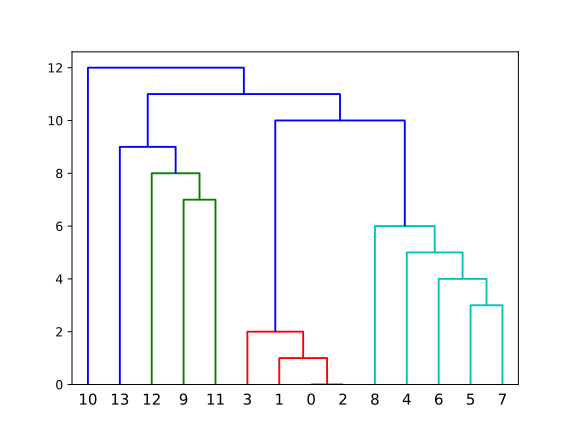
\includegraphics[width=0.49\textwidth]{img/extract_ex_dendro.png}
        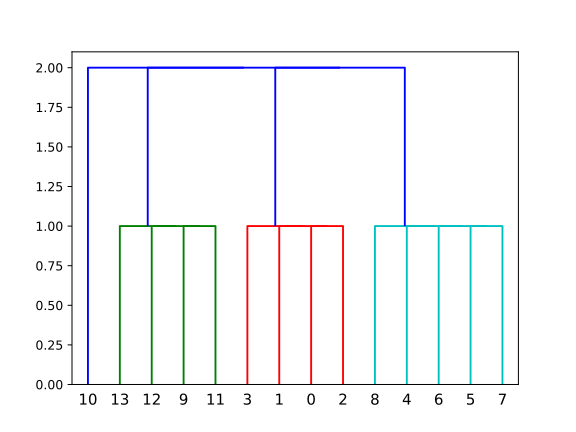
\includegraphics[width=0.49\textwidth]{img/extract_ex_taxo.png}
    \caption{The Input and output of the taxonomy extraction heuristic}
    \label{fig:my_label}
\end{figure} 
 

\section{The Graph-aware Pipeline}
\subsection{Extracting Structural Features}
\subsection{Complexity Analysis}

\section{Implementation Highlights}
For this method i had that challenge "sell yourself"
 
 
